
\section{Theorie}
\label{sec:Theorie}

Ein Laser emittiert Licht, welches durch optische Verstärkung verstärkt wurde. Das emittiert Licht zeichnet sich durch die hohe Intensität, Kohärenz und Geradlinigkeit aus.

\begin{figure}
	\centering
	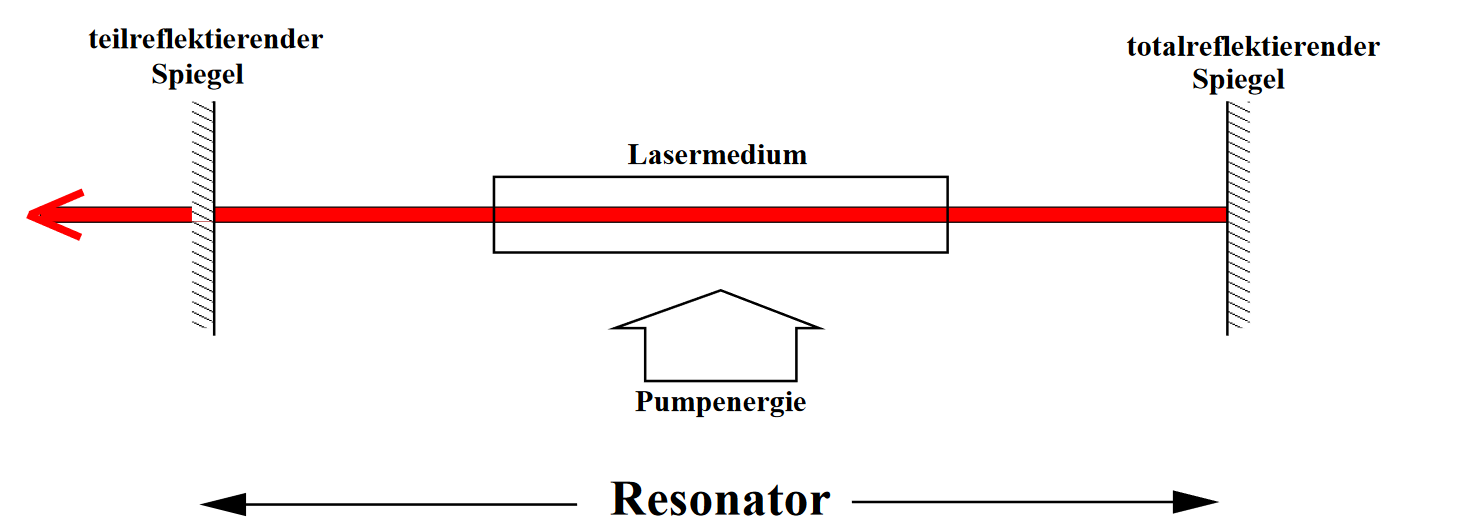
\includegraphics[width=\linewidth-100pt,height=\textheight-100pt,keepaspectratio]{content/Images/schema.png}
	\caption{Prinzipielle Funktionsweise eines Lasers \cite{V61}.}
\end{figure}
Ein Laser besteht im wesentlichen aus einem Resonator, einem Lasermedium und einer zugehörigen Pumpquelle. Das Lasermedium dient dabei zur Verstärkung des Lichtes und der Resonator sorgt für einen effektiv längeren Weg des Lichtes durch das Medium und die Pumpquelle versorgt das Lasermedium mit der für die Verstärkung notwendige Energie. 

\subsection{Der Resonator}
Der Resonator wird durch zwei gegenüber stehende Spiegel realisiert. Mindestens einer der Spiegel lässt etwas Licht durch und sorgt somit dafür, das das Licht den Laser verlassen kann. Bei den Spiegeln kann es sich jeweils um einen plan-parallelen Spiegel oder einem sphärischen Spiegel handeln. Sind beide sphärisch wird der Resonator als sphärischer Resonator bezeichnet und wenn beide plan-parallel sind als plan-paralleler Resonator. Damit der Resonator optisch stabil ist müssen die Verluste geringer sein als die Verstärkung durch das Lasermedium. Dies kann eintreten, wenn die Bedingung
\begin{equation}
	0 \leq \frac{r_1 -L}{r_1} \cdot \frac{r_2 -L}{r_2} < 1 \label{eq:stabil}
\end{equation}
erfüllt ist. Hierbei sind $r_1$ und $r_2$ die Krümmungsradien der Spiegel und $L$ die Resonatorlänge, also der Abstand zwischen den Spiegeln. Damit sich die Stahlen optimal konstruktiv überlagern muss weiterhin die im Resonator zurückgelegte Strecke ein vielfaches von der halben Wellenlänge des Lichtes sein. Diese Bedingung wird auch Resonanzbedingung genannt. Ist diese erfüllt bildet sich eine stehende Welle aus und das Licht wird maximal verstärkt. Um eine nur bestimmte Frequenz zu verstärken kann der Spiegel beschichtet werden, sodass nur diese Frequenz gut reflektiert wird.

\subsection{Das Lasermedium}
\begin{figure}
	\centering
	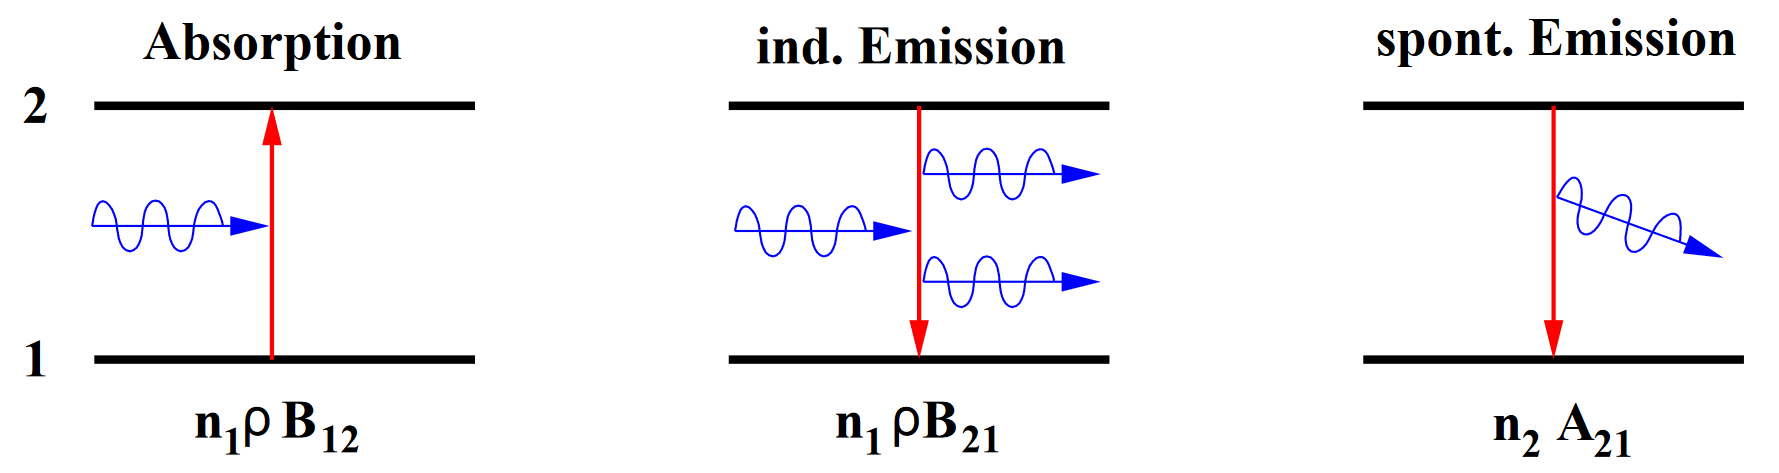
\includegraphics[width=\linewidth-100pt,height=\textheight-100pt,keepaspectratio]{content/Images/emission.png}
	\caption{Schemata für die Absorption und Emission bei einem 2-Niveau System \cite{V61}.}
\end{figure}
Das Lasermedium hat im einfachsten Fall einen angeregten Zustand und einen Grundzustand. Ein Photon hat nun drei Möglichkeiten diese Zustande zu beeinflussen. Einmal indem ein Photon mit entsprechender Energie absorbiert wird und damit für einen Übergang auf das höhere Niveau sorgt (Absorption). Eine andere Möglichkeit besteht darin, dass das höhere Niveau spontan in das niedrigere Niveau übergeht und dabei ein Photon entsprechender Energie freigibt (spontane Emission). Jedoch ist es auch möglich, dass ein Photon mit der Energie des Energiedifferenz der Niveaus den Übergang vom höheren Niveau in das niedrigere Niveau stimuliert (indirekte Emission). 
Das besondere bei der indirekten Emission ist, dass das stimulierte Photon die selbe Ausbreitungsrichtung, Phase und Energie wie das stimulierende Photon besitzt. Dies ist der grundlegende Effekt der für einen Laser genutzt wird. In einem realen Lasermedium handelt es sich bei den verschiedenen Niveaus um die Besetzungsniveaus der Elektronenschalen der Atome. Damit es zu einer Verstärkung des Lichtes kommen kann muss mehr indirekt als emittiert werden als absorbiert wird. Da beide Prozesse gleich Wahrscheinlich sind kann dies durch eine höhere Besetzung des angeregten Zustandes als des Grundzustandes erreicht werden. Jedoch ist dies im thermischen Gleichgewicht nicht der Fall. Um dies dennoch zu erreichen muss durch Pumpen eine Besetzungsinversion geschaffen werden.

\subsection{Die Pumpquelle}
\begin{figure}
	\centering
	\def\svgwidth{0.5\linewidth}
	\import{content/Images/}{5074.pdf_tex}
	\caption{Niveauschema eines Helium-Neon-Lasers \cite{VHeNeGoettingen}.}
\end{figure}
Das Pumpen kann auf verschieden Arten realisiert werden. Beim HeNe-Laser wird zum Pumpen das Helium durch Anlegen einer Hochspannung zur Gasentladung gebracht. Dadurch wird das Helium in einen relativ langlebigen angeregten Zustand gebracht. Durch Stöße des angeregten Heliums mit dem Neon wird die Anregung auf das Neon durch Stöße zweiter Art übertragen und sorgen somit für eine Besetzungsinversion des Neons. Es ist dabei zu beachten, dass das Lasermedium mindestens drei verschiedene Niveaus besitzen muss damit eine Besetzungsinversion möglich ist.


\subsection{TEM-Moden}
Die Resonanzbedingung wird von mehreren Frequenzen erfüllt, sodass mehrere verschiedene Moden möglich sind. Die Moden werden bei einer zylindrischen Symmetrie werden mit $\text{TEM}_{plq}$-Mode ($text{TEM}=\text{transverse electromagnetic}$) bezeichnet. Die Ordnung der Mode wird in radialer Richtung mit $p$, in Winkelrichtung mit $l$ und entlang der Symmetrieachse (in $z$-Richtung) mit $q$ bezeichnet. Für die Intensität der Moden gilt
\begin{equation}
	I_{plq} = I_0 \cos^2 (l \varphi) \rho^2 \left[L_{p}^q\left(\frac{(2 \rho)^2}{1+Z^2} \right)\right] ^2 \exp\left(-\rho \right),
\end{equation}
wobei $L_{p}^q$ ein Laguerre-Polynom, $\rho=2 r^2 / w^2$, $w=w_0 \sqrt{1+\left(\frac{z \lambda}{\pi w_0^2}\right)^2}$ und $w_0$ der minimale Strahlradius ist.

Falls die Symmetrie durch z.B. Brewsterfenster gebrochen wird, um ein polarisiertes Licht zu erhalten, werden die Moden mit  $\text{TEM}_{mnq}$-Mode bezeichnet. Die Ordnung der Moden in $x$- und $y$-Richtung werden mit $m$ und $n$ bezeichnet. Für die Intensität der Moden gilt nun
\begin{equation}
I_{mnq} = I_0 \left(\frac{w_0}{w}\right)^2 \left[H_m\left(\frac{\sqrt{2} x}{w}\right) \exp\left(\frac{-x^2}{w^2}\right) \right]^2 \left[H_n\left(\frac{\sqrt{2} y}{w}\right) \exp\left(\frac{-y^2}{w^2}\right) \right]^2, \label{eq:tem}
\end{equation}
wobei $H_m$ ein Hermitesches Polynom ist.


In beiden Fällen gilt für die $\text{TEM}_{00q}$-Mode
\begin{equation}
I_{mnq} = I_0 \exp\left(-\frac{2 r^2}{\omega ^2}\right). \label{eq:gaus}
\end{equation}

\subsection{Intensität von polarisierten Licht hinter einem Polarisationsfilter}
Ein Polarisationsfilter lässt nur eine Polarisationsrichtung passieren. Falls das Licht vorher um ein um einen Winkel $\delta\phi$ verschiedenen Winkel polarisiert ist als der Polarisationsfilter passieren lässt gilt für die Intensität des Lichtes hinter diesem
\begin{equation}
	I=I_0 cos^2(\delta\phi), \label{eq:polar}
\end{equation}
wobei $I_0$ die Intensität vor dem Polarisationsfilter bezeichnet.

\subsection{Zusammenhang zwischen dem Beugungsmuster eines Gitters und der Wellenlänge des gebeugten Lichtes}
Durch das Einbringen des Gitters in den Lichtstrahl wird dieser am Gitter gebeugt. Dies führt zu Interferenzeffekten hinter dem Gitter. Es bilden sich Intensitätsmaxima aus. Aus den Abständen zwischen diesen und dem Abstand zum Schirm kann die Wellenlänge des Lichtstrahles folgendermaßen bestimmt werden
\begin{equation}
	\lambda = \frac{g \sin(\arctan(x/b))}{n}, \label{eq:lambda}
\end{equation}
wobei $g$ die Gitterkonstante, $x$ den Abstand des Hauptmaxima der Ordnung $n$ zur optischen Achse des ursprünglichen Strahles und $b$ der Abstand zwischen dem Schirm und dem Gitter ist.



